\chapter{Introduction}
\label{ch:introduction}

\section{Motivation}
\label{sec:motivation}
Computers and computing devices are becoming an essential part of our lives day by day.  The increasing demand for such computing devices increased the necessity of comfortable and practical computer interfaces.  The number of systems using vision-based interaction and controlling mechanism exponentially increased in the last decade.  As a result of this, gesture recognition got more and more popular in the research community due to various application possibilities in human-machine interaction. Compared to Mouse and keyboard, any vision-based interface is more convenient, practical and natural because of the intuitiveness of gestures.   In Cambridge  Dictionary\footnote{\url{https://dictionary.cambridge.org/dictionary/english/gesture-recognition}}, gesture recognition is defined as the ability of a computer to react to movements made by a human being and to do tasks according to what the movements mean.  In other words, gesture recognition is a natural user interface for human-machine communication that allows computers to capture and interpret human gestures.\\

In order to understand gesture recognition, we need to define what gesture is. A gesture is a form of non-verbal communication in which a movement of part of the body is involved to communicate or express an idea or a meaning.  Gestures can consist of movement of the hands,  face, or other visible parts of the body.  In other words, a gesture is a natural interface in human-machine communication for providing real-time feedback to a machine; therefore, it has been the most convenient way to establish this interaction.\\

Gesture recognition can be practiced with mainly three kinds of way:  (1) Using glove- based wearable devices \cite{abhishek_glove-based_2016}, (2)  3D Model-Based Hand method \cite{wen_intraoperative_2010}  and (3) Vision-based Gesture  Recognition.   The first method comes with the obligation of wearing an additional device with which lots of cables comes even though the accuracy and the speed of detection are generally sufficient.  The second, on the other hand, lacks to achieve reasonable time constraints for recognition although it can classify and detect hand gestures correctly.  Lastly, in (3) an image capturing sensor has been used , such as camera, infrared sensor or depth sensor; which is much more practical and intuitive. Since the user does not require to wear a burdensome device together with its acceptable accuracy in recognition and speed in computation, this option stands out as the most practical one.  It is essential for the infrastructure of any gesture recognition system to be practical.  After all, we aim to use it in a real-life environment\\

On the other hand, the progression of Artificial Intelligence (AI)  brought up many possibilities in many research areas.  Computer vision is one of the most affected areas especially after the development of convolutional  neural networks (CNNs).  Before CNNs, it was common to train classical machine learning algorithm  (e.g., SVM, Regression, K-Means) on hand-crafted features from images. Moreover, the challenge was how to extract the best representative features in the CV community.  This approach has been investigated in the area of action recognition \cite{shen_dynamic_2012,tamrakar_evaluation_2012,wang_robust_2015}.   Since gesture/action recognition has strong relationships with both spatial and temporal information, reserachers investigated how to represent shape, appearance,  and motion cues using traditional computer vision techniques.  Some video classification systems successfully employ improved dense trajectories  \cite{wang_robust_2015} and Fisher vector representations \cite{perronnin_improving_2010} , which are widely regarded as state-of-the-art local features and aggregation techniques for video analysis.\\

As opposed to hand-crafted features, there is an irrefutable demand for feature representations learned by deep neural networks (DNNs).  CNNs has been studied and proven as a useful feature extraction tool for many image-based tasks.  The increased number of available large datasets has also played a crucial role for these data-hungry models.  Currently, CNNs provides the state-of-the-art results for image recognition, segmentation, tracking,  and classification tasks.  Consequently,  it does not  surprise  that  CNNs is also dominant in video-based tasks,  such as gesture  recognition and  action  tracking.   Especially after development of different version of CNNs, such as R3DCNN \cite{molchanov_online_2016}, ResNet  \cite{hara_can_2017} and  C3D \cite{tran_learning_2014}, that  can capture  not  only spatial  but  also temporal information  out of a stack of images.\\


Most of the previous researches mainly focus on increasing the offline accuracy in gesture recognition, and some are almost impossible to run in real-time because of the computational limitations on the calculation of the modalities they used such as optical flow even though these models can achieve the best performance.  However, in real-time applications, the ability to have a fast processing model is as important as the level of the accuracy.  In real-time  gesture recognition applications, there are three crucial characteristics need to be satisfied by the system:
\begin{enumerate}
\item Accuracy
\item Fast reaction time
\item Resource efficient
\end{enumerate}
Most of these works, only consider (1), and disregard others. Consequently, research community lacks a blueprint that describe how to efficiently integrate these models into an online working system.\\

In this work,  a novel strategy that allows us to integrate these models, which shows an acceptable accuracy performance,  into a real-time application as efficient as possible. The proposed architecture contains two offline-trained CNN archotecture, a gesture classifier (classifier)(classifier)\footnote{In this thesis, this model is referred as "classifier"} and a light weight detection classifier (detector)\footnote{In this thesis, it is referred as "detector"},  which identify between gesture and no gesture. By this way, we can achieve followings:
\begin{itemize}
\item Compensation  of the variability  in the number of frames in the gestures
\item Reduction  of noise due to the movement of the subject, e.g., walking, or random hand motions
\item Efficient use of computational resources because the classifier, which is a much more complex model than the detector, runs only when a gesture is detected. 
\end{itemize}

Additionally,  according to Molchanov et al.  \cite{molchanov_online_2016}, dynamic hand gestures generally consists of overlapping phases:  preparation, nucleus, and retraction,  of which the nucleus is most discriminative.   The other two phases can be very similar for different gestures, and the actual information for the gesture lies in the nucleus phase.   On the other hand,  in \cite{card_information_1991,miller_response_1968} it is stated that humans get annoyed with lags greater than 100 ms in reaction time. As a results of this, we propose several post-processing methods that allow offline-trained models even to detect/classify gestures while still in the nucleus phase.   To the best of our knowledge, the only work done on this is \cite{molchanov_online_2016} and they do not use any pre-trained models instead they train a model using CTC  loss, and this is not applicable for our purposes since we aim to use an already working model not training one. Moreover, our goal is to identify dynamic gestures not only with negative lag but also do single-time activation per gesture in real-time.\\

In the rest of this chapter, I give an introduction to computer vision and the evolution of action and gesture recognition. After that I  give more detail about Machine Learning and its effect in computer vision tasks, and finally I introduce the development of CNNs and different variations of it.\\
\clearpage
\section{Computer Vision}
\label{sec:CV}

Computer  Vision (CV) is a multidisciplinary field that deals with the process of using machines/computers to extract high-level information by processing digital images and videos.  Information in this context means symbolic (numerical)  descriptors of the real world projected onto 2D space.  CV utilizes models constructed with the help of geometry, physics, mathematics, statistics, machine learning, and learning theory.\\

The history of computer vision goes back to 1966. It started as an undergraduate project \cite{papert_summer_1966} at the Massachusetts Institute of Technology.  This project aimed to create an intelligent algorithm that recognizes objects using a camera to help a robot. After this first attempt, in the following decade, researchers invented algorithms like optical flow, edge and corner detection,  which are still actively been used in the domain even now, formed the primary foundation of the computer vision. Also, it has been followed by more complex mathematical methods such as projective 3D reconstructions, and camera calibration.  One of its main application areas is vision-based gesture recognition,  especially hand gesture recognition. \\
%One common approach to deal with gesture recognition is utilizing some mathematical algorithms in computer vision, such as  optical flow, as a feature extractor from images. Another method is creating 3D Model-Based Hand method  \cite{wen_intraoperative_2010} that aim to create a 3D model of each gesture and detect gestures by using a distance measure between the 3D reconstructed data from a test image with the true model of gestures.

As a scientific field, computer vision has been used in many challenging tasks in image and video domain.  Some of these are :
% 3D reconstruction, image segmentation, scene reconstruction, object recognition in images, image restoration, action / gesture recognition, surveillance monitoring, autonomous driving, event detection, etc.  
\begin{itemize}
\item Video \textbf{motion analysis}, algorithms producing information based on the apparent motion in the temporally related images like the velocity of objects, or the camera itself.
\item \textbf{Image segmentation}, algorithms dividing a digital image into multiple sets of views.
\item \textbf{Scene reconstruction}, algorithms  that  infer the geometrical  structure of a scene inputted through  a collection of images.
\item \textbf{Image restoration}, algorithms  that  remove the  noise from a corrupted/noisy image and estimate  the original image. 
\end{itemize}
Additionally, it is important to note that, unlike digital image processing,  computer vision aims to retrieve three-dimensional pieces of information from images and have a full understanding of the scene.\\
\begin{figure}[t]
	\centering
	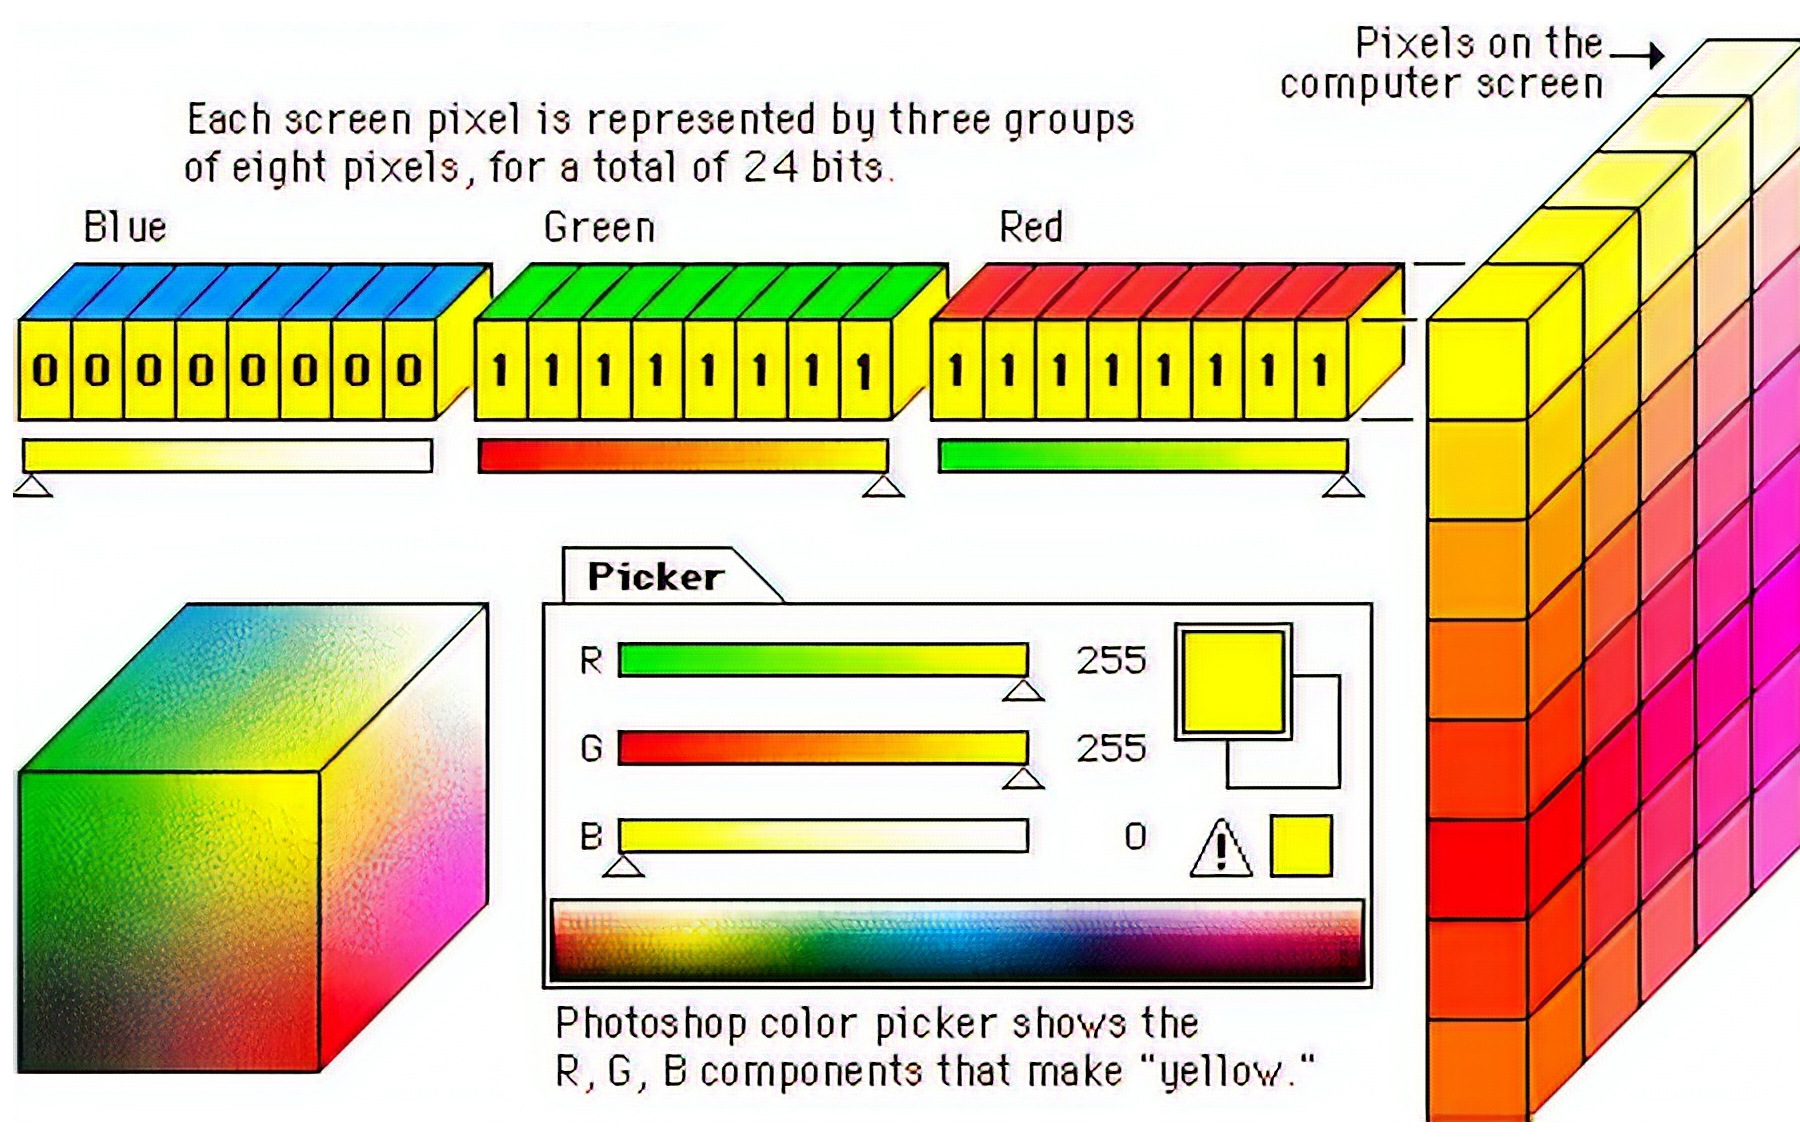
\includegraphics[width=0.8\linewidth]{figures/rgb}
	\caption{RGB color representation in 24-bit color display}
	\label{fig:rgb}
\end{figure}

In order to comprehend the broad range of computer vision, we shall understand the way computers "see" an image. Computers represent everything by binary numbers, meaning that it only consists of 0 and  1.  So images are no exception.   Machines interpret images as a series of pixels, each with their set of mathematical equivalent of color values as numbers.   In other words, an image is represented by a matrix, and each item in this matrix corresponds to a pixel; and the value of an item,  pixel in this context, represents the color values.  One can represent colors with numbers in many ways.  The most common method is to represent the level of red, green, and blue primary colors. By changing the respective amount of these colors, any desired color can be created. Each of these primary colors is represented by a 2-dimensional matrix of $height \times width$, in which each item represents the amount of the color in the corresponding pixel.\\

The range of colors is limited by the amount of bits assigned to each item.  If it is 8-bit, then we can have values ranging from 0 to 255 for each of the RGB primaries of the color, and in total, we can have 2563 = 16, 777, 216 different color combinations. Figure \ref{fig:rgb}\footnote{\url{https://cdn-images-1.medium.com/max/1600/0*I6XPXr9fzJ43L0ii.gif}} shows the way colors represented by machines.\\

As the involvement of machines in our daily lives escalated, human-computer interaction (HCI)  techniques became the main challenge for the computer vision community.   A typical example of these is controlling machines with commands performed by hands. As expected, image-based hand gesture recognition interfaces \cite{pavlovic_visual_1997} got popular really fast.  In the early years of computer vision, this had been done by creating models/templates of hands position and motion similar to many other applications of computer vision like object recognition.  Then it followed by extraction  of features using these templates.  And finally, an intelligent trajectory/motion recognition algorithm  used for classification \cite{jiang_dynamic_2013}. An example of this general form is shown in Figure \ref{fig:cv_gesture_workflow}.\\

\begin{figure}[h!]
	\centering
	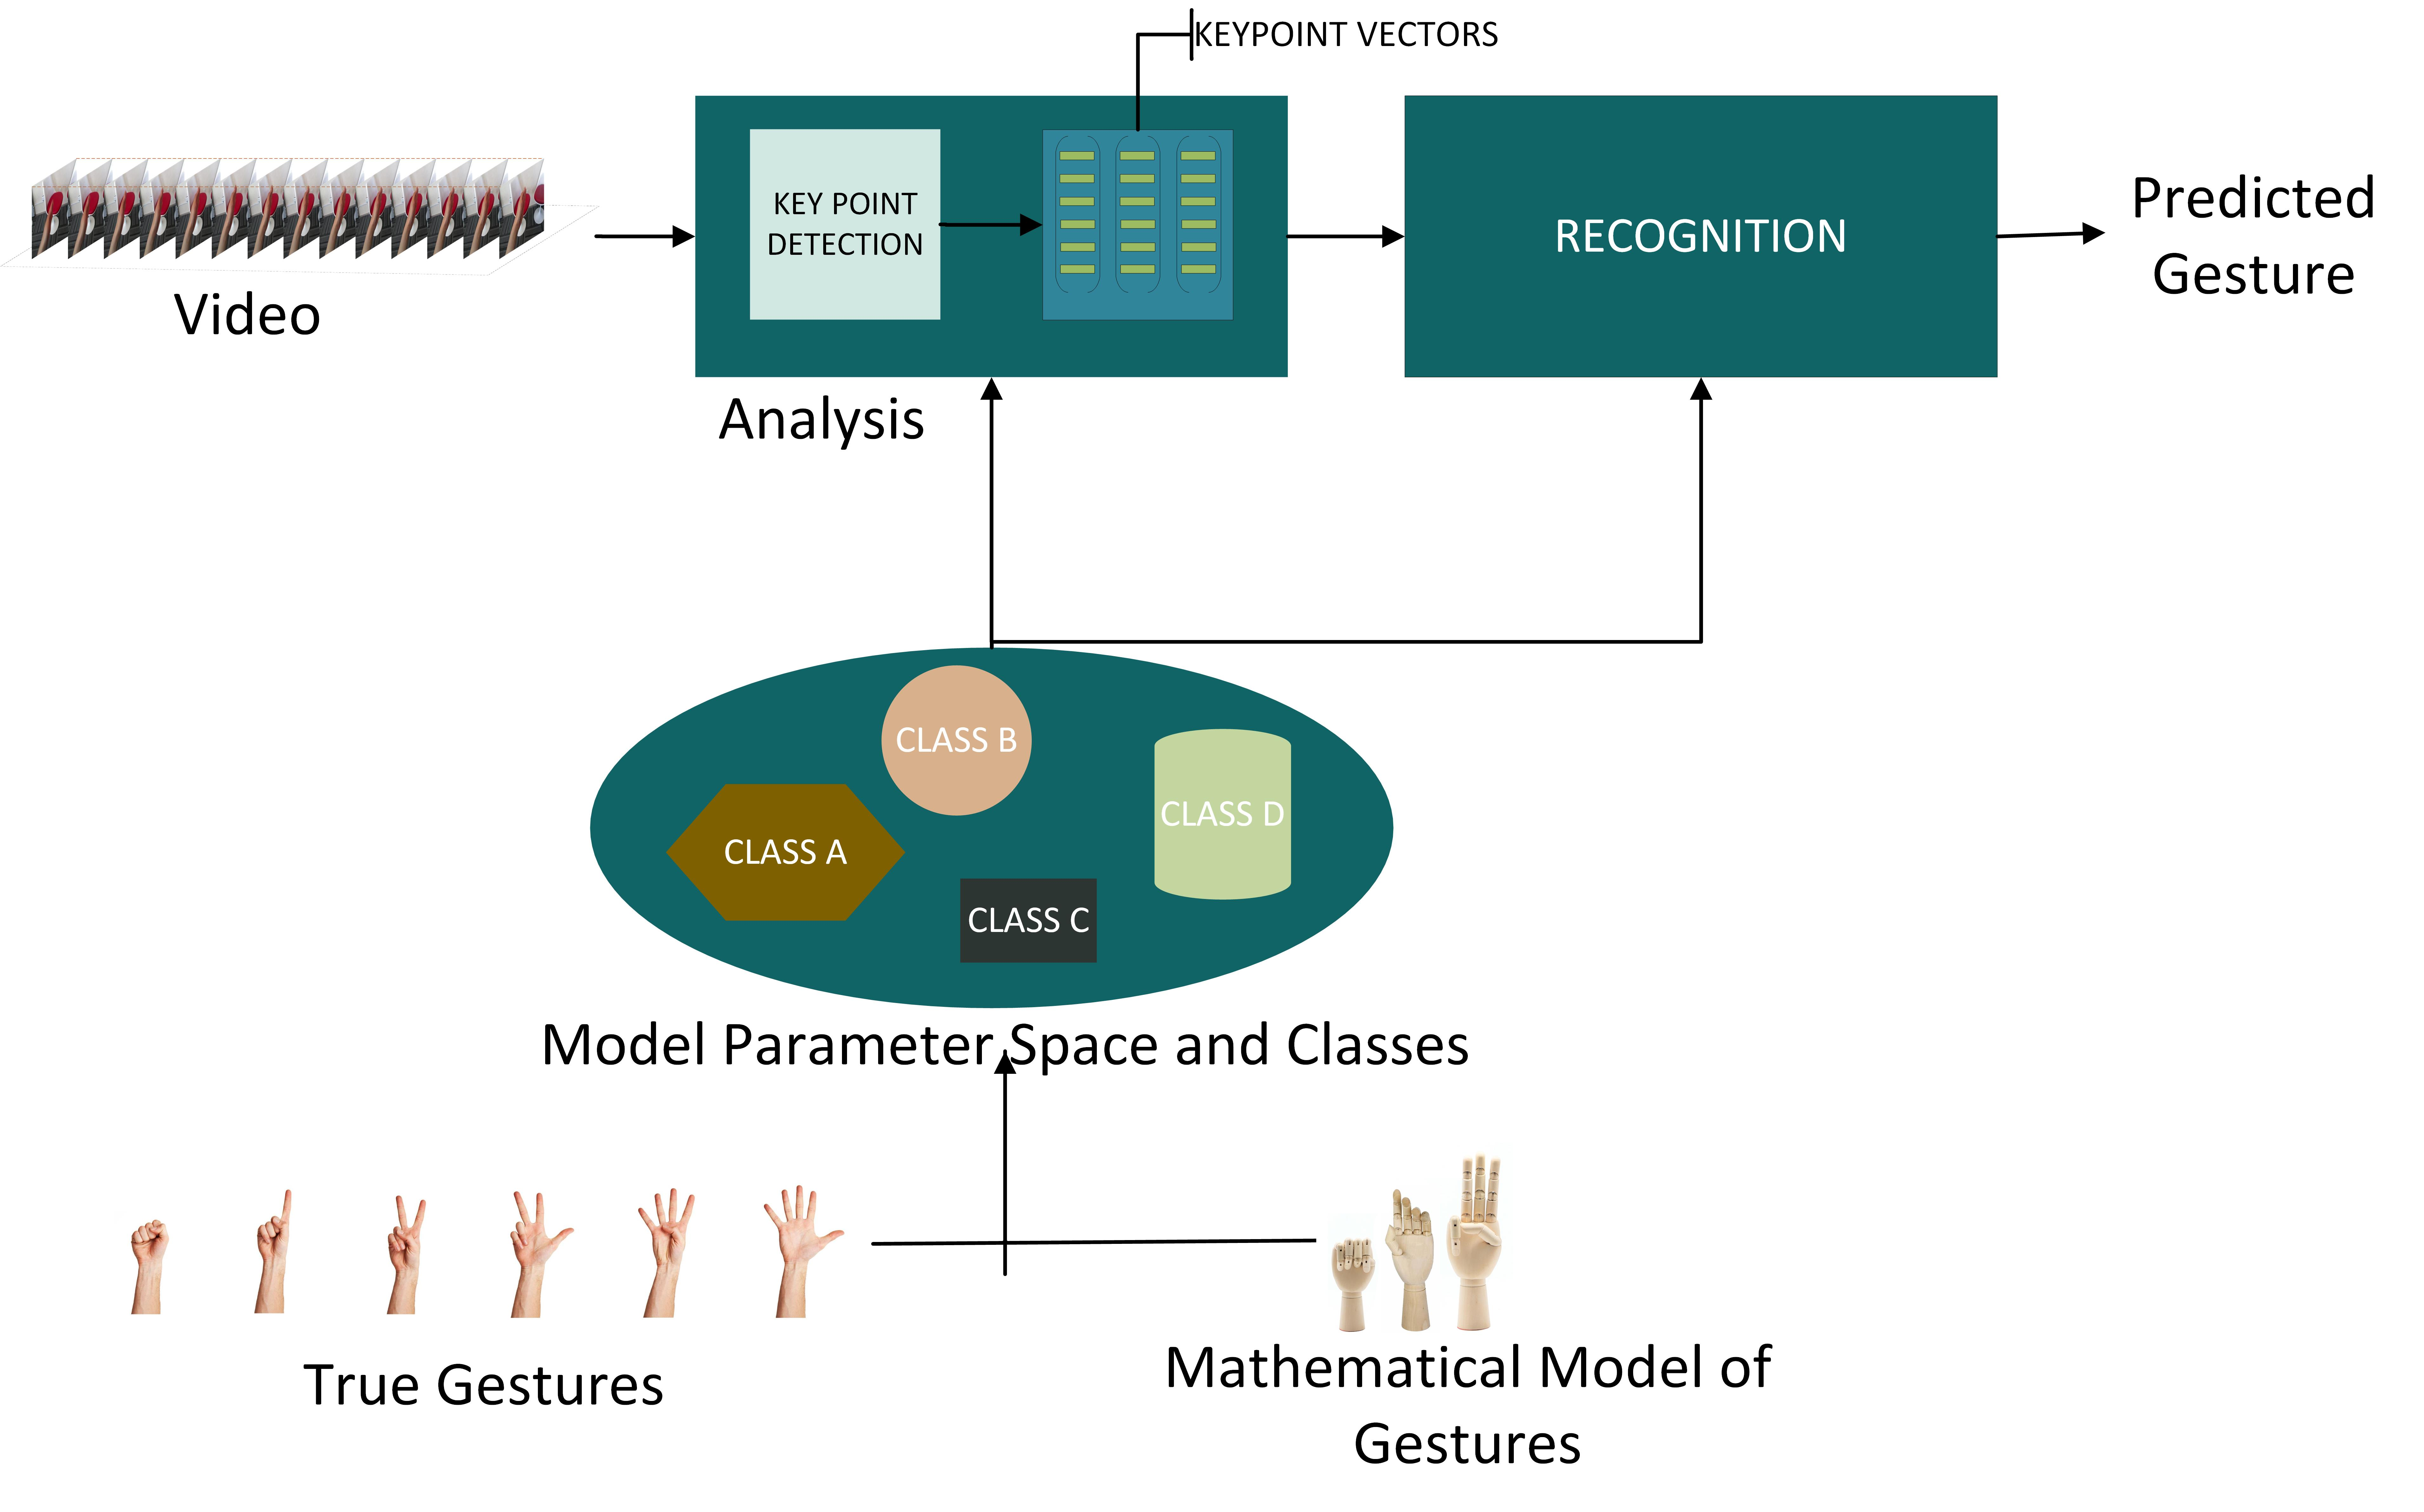
\includegraphics[width=0.8\linewidth]{figures/cv_gesture_workflow}
	\caption{A general framework of traditional gesture recognition system:  Each frame from the video stream is analyzed, and it is converted to a model space of the gestures.  After then  a recognition algorithm,  mostly k-means, predict  observed gesture.}
	\label{fig:cv_gesture_workflow}
\end{figure}

Although this approach showed some level of success, it is far from perfect.   For example, hand configuration is not always the same and has more than  26 degrees of freedom, and hand shape can change drastically depending on the view of the camera \cite{bergh_haarlet-based_2009}. One major drawback of this approach is that it is built upon many assumptions which have been taken for granted,  and either not general enough or too specific to the task.  Additionally,  computation requirements for most of these algorithms do not allow a robust real-time application system.  For a detailed background of computer vision researches on hand gesture recognition, please see Chapter  \ref{ch:relatedwork}.  These drawbacks brought up the question: "How  can we have a more reliable and robust algorithm for computer vision applications,  especially for the feature extraction phase?" With the availability of large datasets and the development of new computational devices like Graphical  Processing  Units  (GPUs),  it became possible that deep learning methods to show their true potential.   Consequently, conventional computer vision methods have been partly replaced by Deep Neural Networks in many application areas lately,  especially after the CNNs had proven their abilities in learning feature representations from images through the large publicly available datasets.\\

\section{Machine Learning} 
\label{sec:ML}

Machine learning is an application of Artificial  Intelligence  (AI)  which enables systems to automatically find patterns from the seen data without being preprogrammed.  Artificial neural networks (ANNs) or other methods of machine learning are mainly supervised technologies.  This means that, in addition to a large amount of input data, a substantial (best case equivalent) amount of corresponding labels is needed for this input data in order to sufficiently characterize the properties of the input data.  Those labels enable the machine learning method to find a meaningful connection between input data and its labels.  The general workflow of supervised machine learning task is illustrated in Figure \ref{fig:svml}: In (a) Training, the aim is to learn a classifier model function.In (b) Prediction,  the learned classifier model (output function of the machine learning algorithm)  can be used to classify new, previously unseen input data. The output/prediction of this classifier is a label for the new, previously unseen input. The portion of correctly classified input data gives the accuracy of the classifier model.\\
\begin{figure}[h]
	\centering
  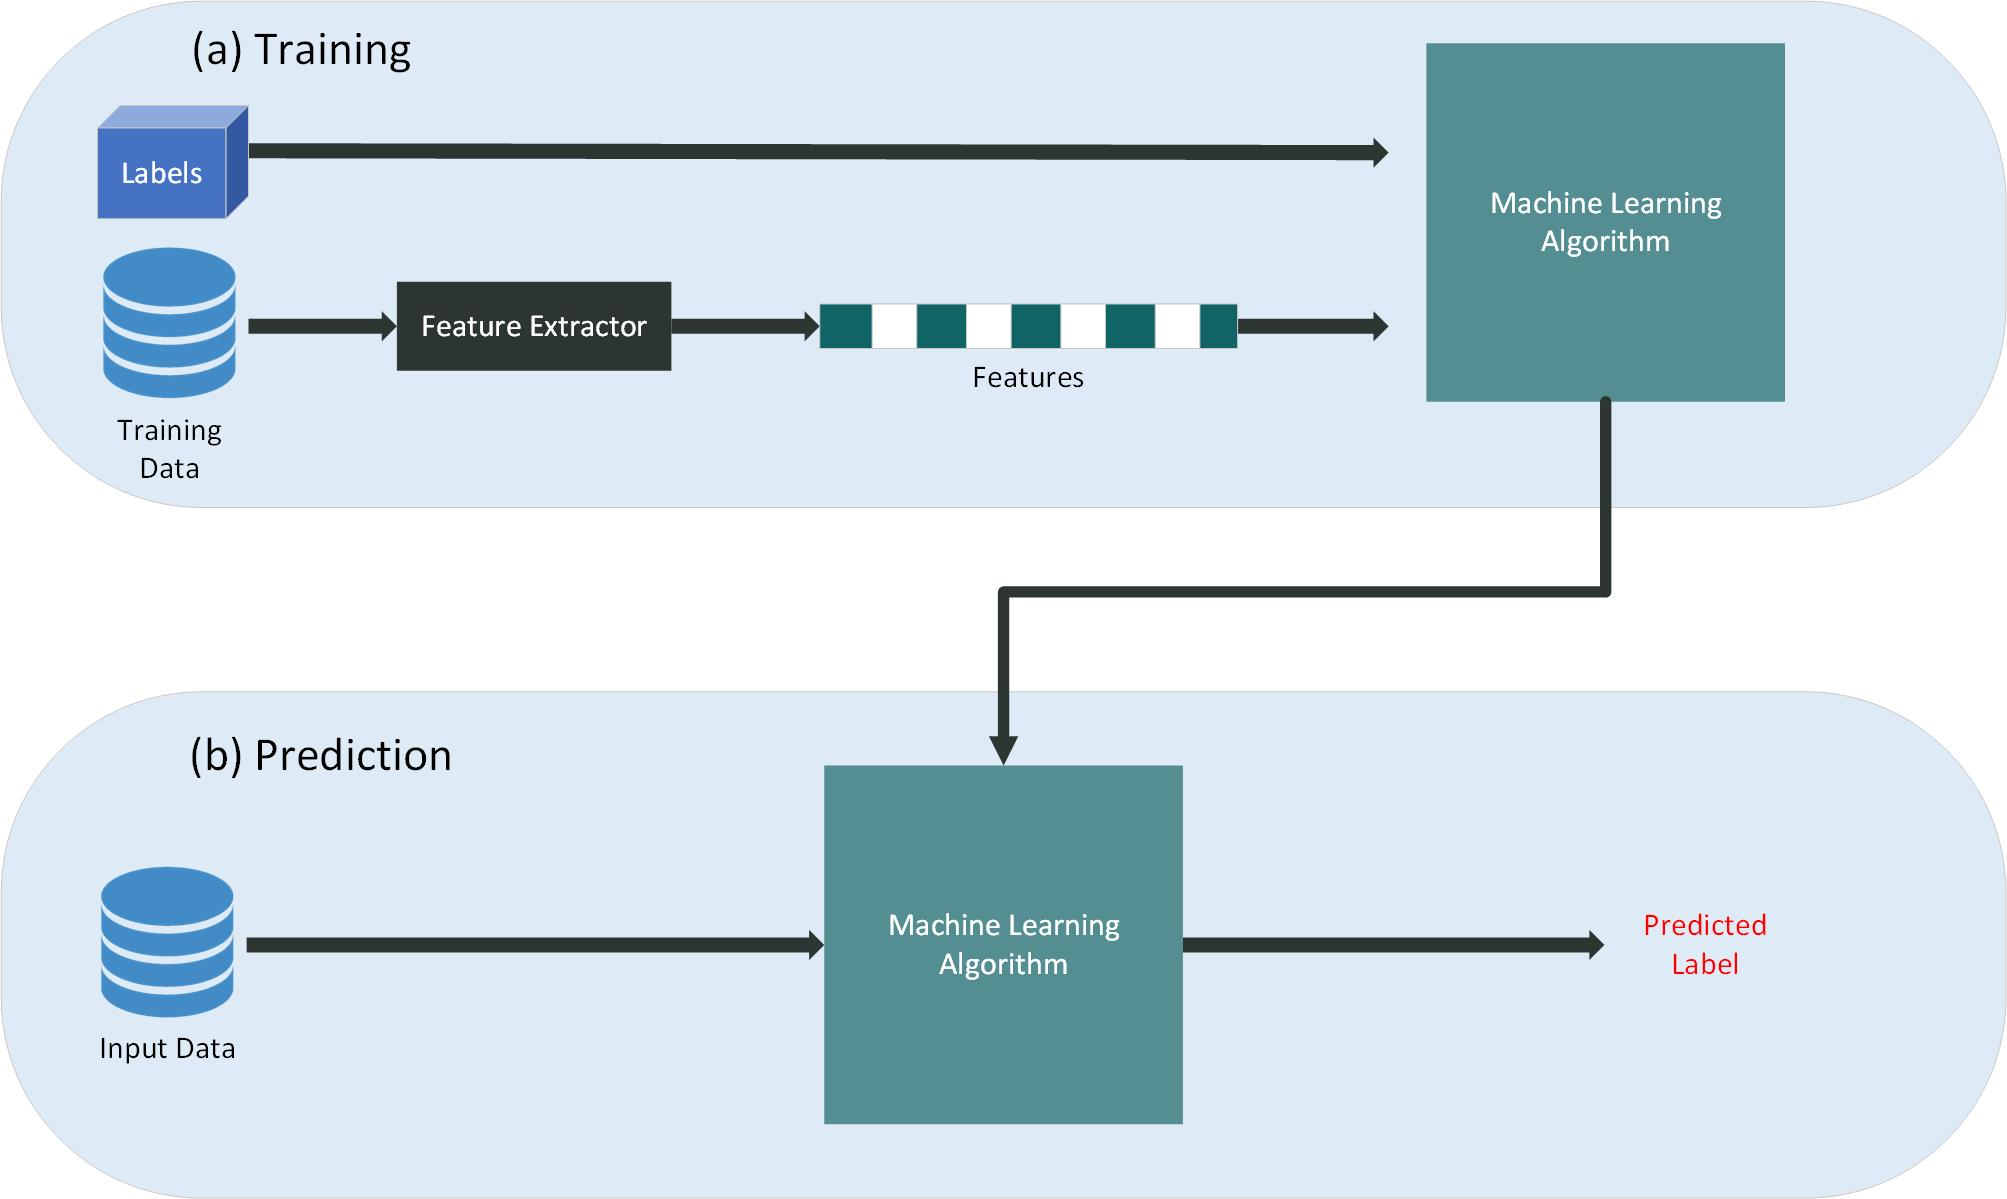
\includegraphics[width=\linewidth]{figures/ml_workflow}
  \caption{Supervised Machine Learning}
  \label{fig:svml}
\end{figure}

The concept of inferring a function from labeled training data,  which is described in the paragraph above and illustrated in Figure  \ref{fig:svml}, is called Supervised Machine Learning.  Methods of supervised machine learning include (among many others) regression, trees, random forests, nearest neighbor algorithms,  SVM (Support  Vector Machines), artificial neural networks, and many methods of deep learning, e.g. Convolutional  Neural Networks (CNNs), Long-Short-Term-Memory Networks (LSTMs),  or Neural Turing  Machines (NTM).\\

Apart from supervised machine learning, unsupervised machine learning (without labels) allows for finding patterns in the data,  also referred to as clustering.  Also, there is a third method; one can combine supervised and unsupervised learning methods if the small portion of the input data is labeled and the rest is unlabeled.  In a first step, patterns in the input data  are detected  in an unsupervised manner.  In a second step, the generated data pattern model is used as a pre-trained-model and labels, which are only available for a small portion of data set,  are used to add meaning to the previously structuring pre-trained model.   This method is called Semi-supervised learning,  see Figure  \ref{fig:ssml}. However,  for gesture recognition tasks,  - to the best of our knowledge- we almost always know the labels for the data in the training phase.   So, in this work,  we considered supervised learning.\\
\begin{figure}[h]
	\centering
  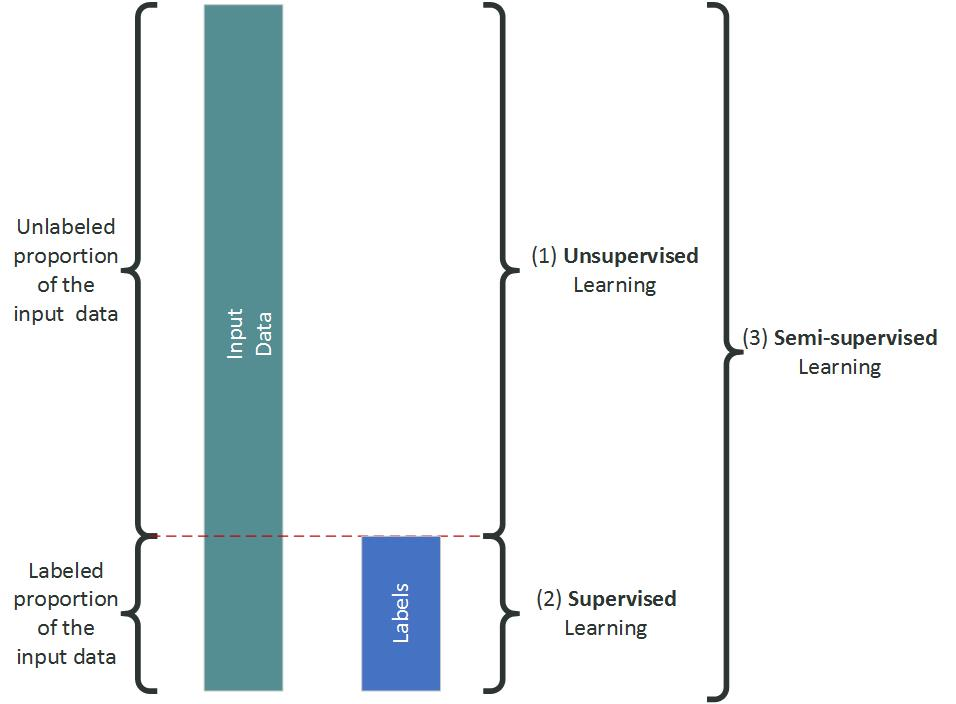
\includegraphics[height=0.6\linewidth]{figures/ml_learnings}
  \caption{Semi-Supervised Machine Learning for partly-labeled input data}
  \label{fig:ssml}
\end{figure}

Methods of Machine Learning are currently broadly used in a variety of sectors, also often referred to as methods of ”Artificial  Intelligence”  (AI).   Popular areas of application are, e.g., automatic image recognition,  automated driving or precise weather forecasts. Analysts evaluated AI’s potential as very high being a game changer for the technology of the 21st Century of humankind.  Naturally, computer vision has shared its part of the change, and in the last decade many computer vision tasks have been strengthened, evolved with the integration of more intelligent algorithms.  Convolutional  neural networks (CNNs) and its variations played an important part in this.  CNNs are being known for their ability in learning feature representations with a much lower number of parameters as opposed to the traditional fully-connected neural network.   As a consequence of this,  ”old-fashioned”  methods have been used in CV has been replaced by a CNN network.  In other words, the analysis and recognition parts in Figure \ref{fig:cv_gesture_workflow} are replaced by a machine learning algorithm, usually, a CNN network followed by a fully-connected network or LSTM network.\\


\subsection{Feed Forward Neural Networks}
\label{subsec:ffnn}
Artificial neural networks (ANNs) create the basis for many models in machine learning.  It is called ”neural”  because it is a brain-inspired system which is intended to imitate the way that we humans learn.  As a structure, it resembles a lot to the neural structure of human brains.  In some tasks which require mathematical calculations,  ANNs can find patterns which are far too complicated for a human programmer to extract and train the machine to recognize manually.  It consists of computing units called neuron,  and these neurons form a layer at which all neurons output together with a set of weights for one input. Each neuron in a layer is connected to all neurons in the consecutive layer through learned weights, refered as "fully-connected".  Neural networks consist of input,  output and (in most cases) hidden layers.  In Figure \ref{fig:ff}, the basic structure of a neuron and a simple fully-connected two layer networks are shown.\\
\begin{figure}[h]
	\centering
  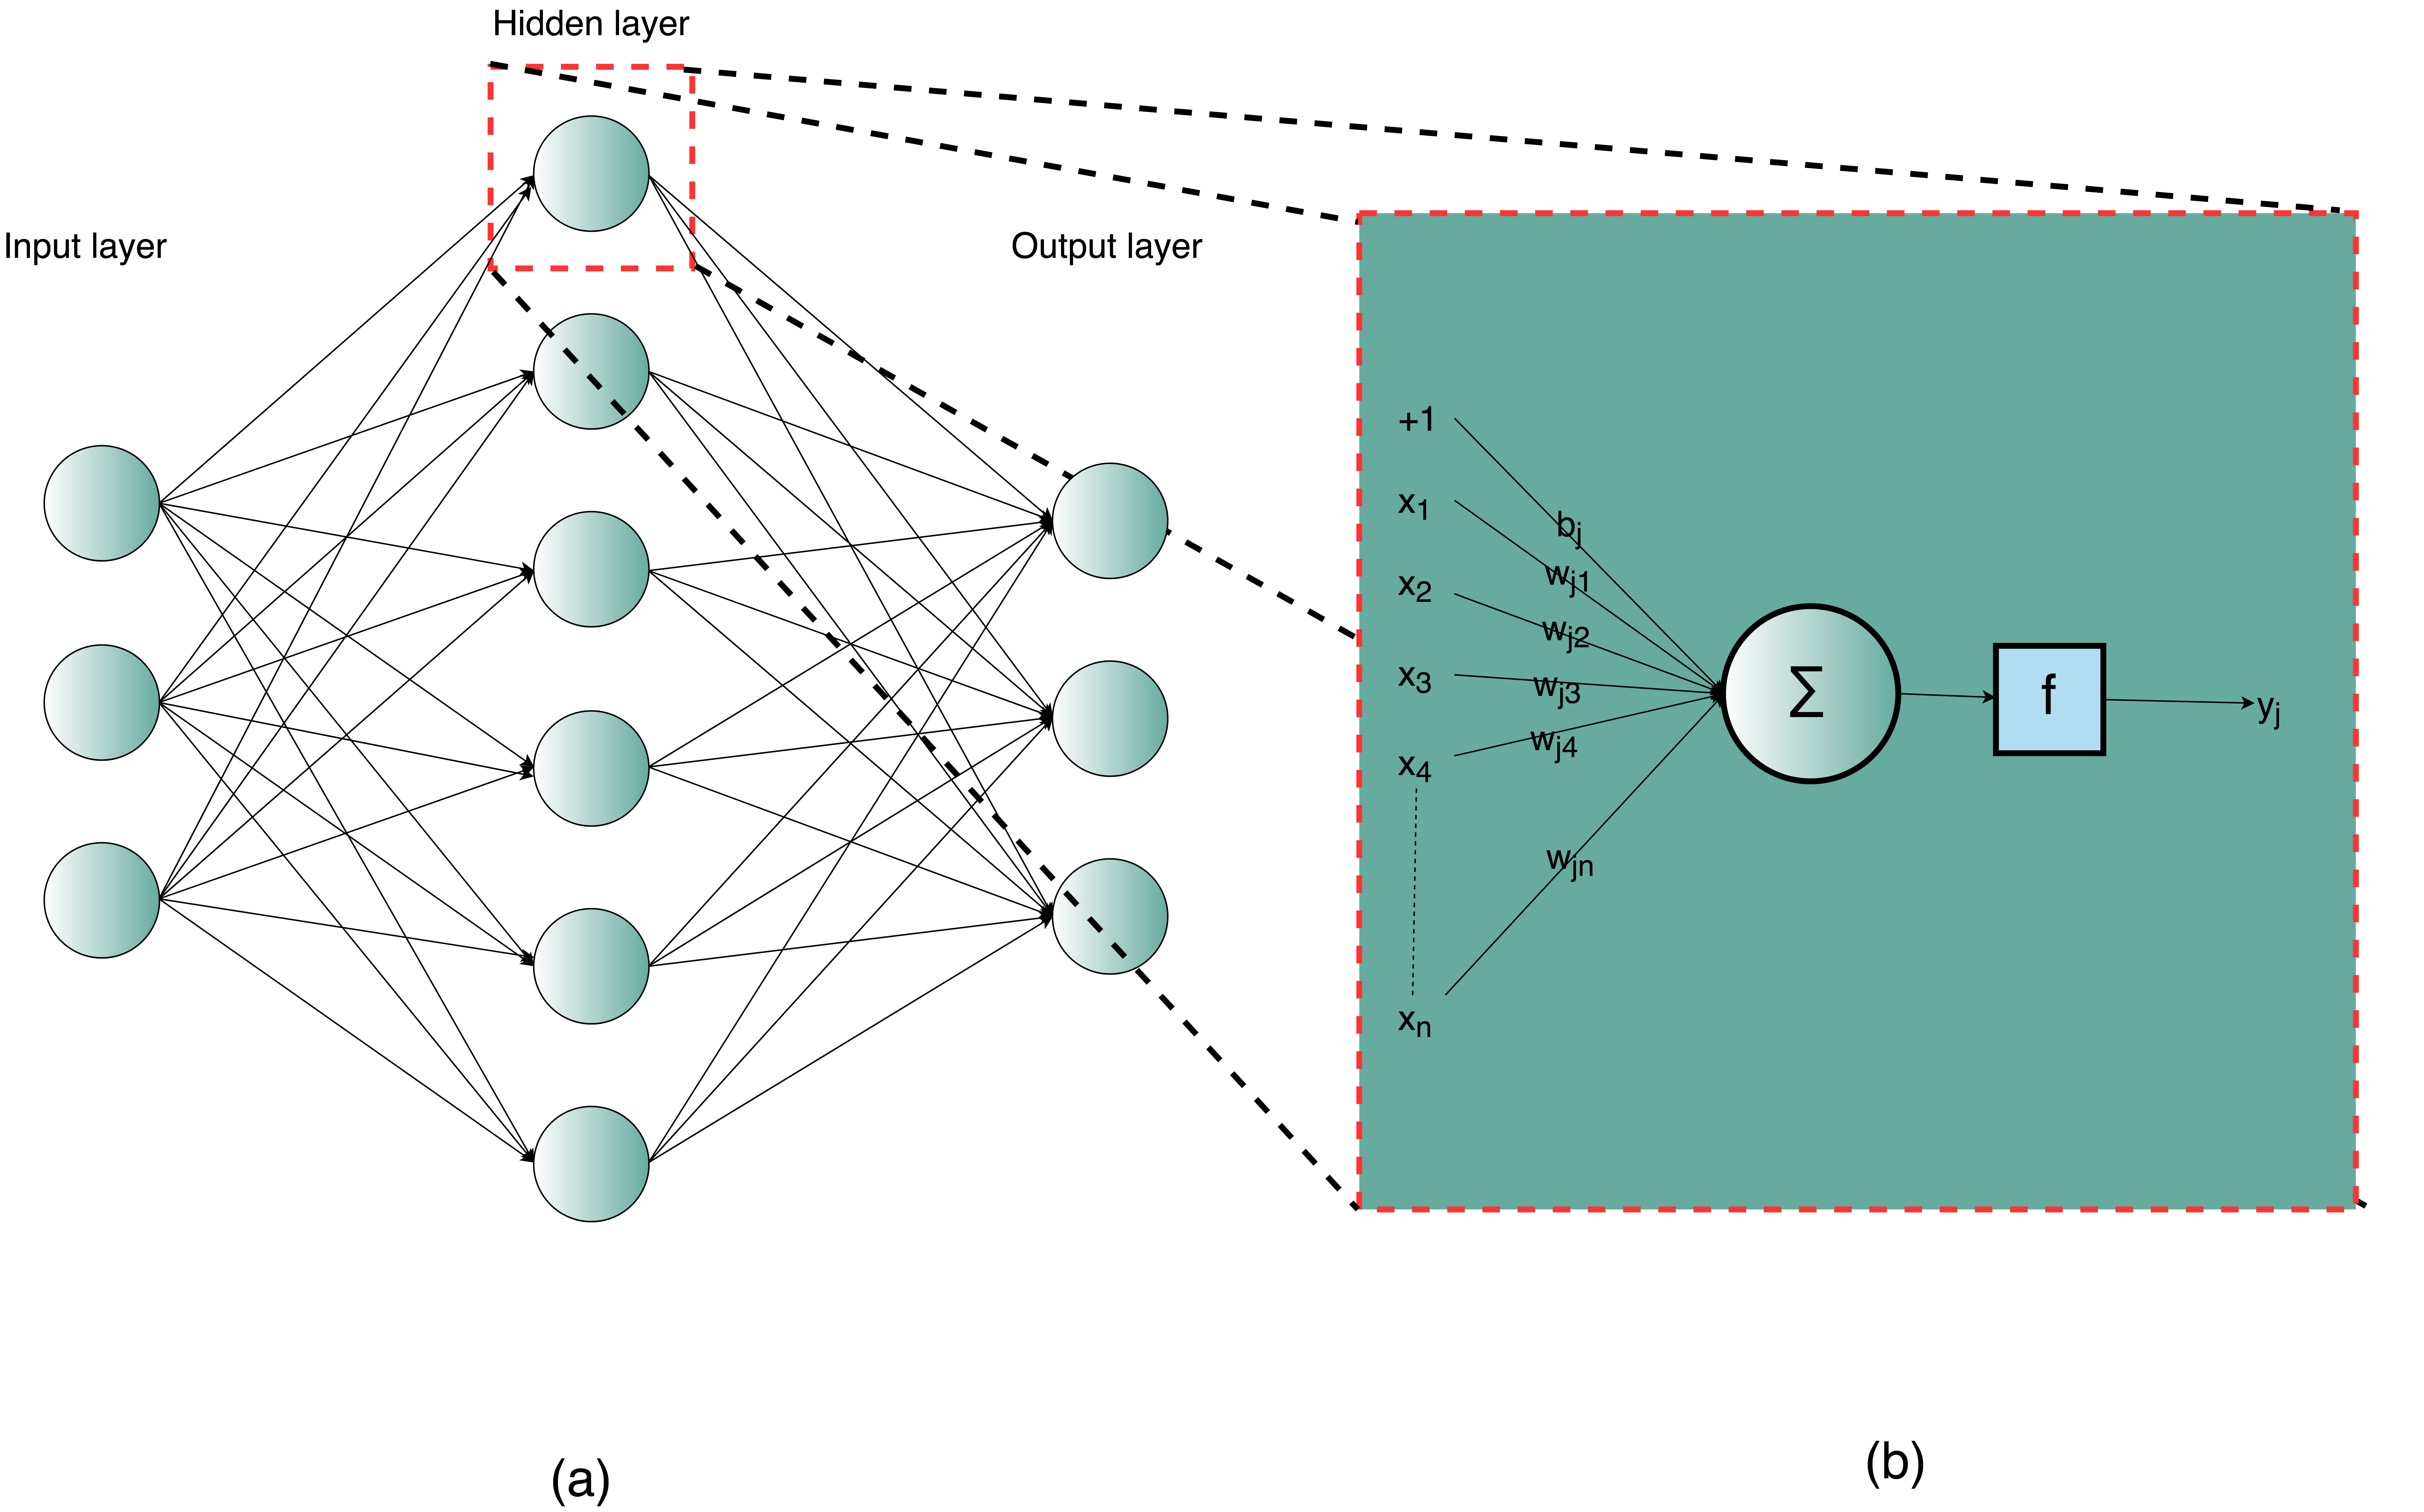
\includegraphics[width=\linewidth]{figures/ff_structure}
  \caption{An example ANNs structure: (a) A two-layer fully connected neural network with one hidden layer and output layer (b)  Structure of one neuron which is fed by n inputs and one bias term  (+1),  which are outputs of the previous layer, and an activation function f.}
  \label{fig:ff}
\end{figure}

Neural networks (perceptrons) roots back to the 1940s. They have become an essential method of artificial intelligence (AI)  in the last decades because of the discovery of the technique called \textbf{backpropagation}, which is derived from the chain-rule of mathematical derivation and allows neurons to adjust their weights according to the distance between the predicted outcome and the true outcome.\\

Another critical factor in the success of neural networks is the technological development in the last decade, which  make it possible to train deeper networks (\textbf{deep learning neural networks}). The most outstanding ability of the neural networks is to automatically learn to extract different features using backpropagation, which allow it to converge to the true label.  If the amount of the data is enough, then it can learn the feature representations without much of intervention by a practitioner. Besides that,  the deeper the neural network is, the better it learns distinctive features.\\ 

The most basic ANN model is the feedforward multilayer perceptron network (MLP) in which each neuron in one layer is connected to each neuron of the following layer \cite{goodfellow_deep_2016}, and these connections do not form a cycle.  This structure is also called a fully-connected neural network. Some other examples of feedforward networks are convolutional neural networks (CNNs) and  recurrent neural networks (RNNs) in which the information flows not only from input to output but also from output to input using feedback connections.  RNNs is a strong tool in complex tasks such as learning handwriting or language recognition in which there are temporal relations.  In this thesis, however, we will focus more on CNNs and their the ability in learning spatiotemporal relations, as we do not aim to desing a complex model that make use of, instead we aim for converting  any pretrained models into a real-time application with the use-case of vision-based gesture recognition.\\

\subsection{Convolutional Neural Networks (CNN)}
\label{subsec:cnn}
Convolutional  Neural Networks (CNNs) is biologically-inspired variants of Multilayer Perceptron (MLP).  It stems from a research in the 1960s on the brain of cats by Hubel and Wiesel \cite{hubel_receptive_1968}.  In order to understand convolutional neural networks we first need to understand how a human brain works.  For over 500 million years, the human brain and the visual system evolved to a system can differentiate and understand the 2-dimensional world and interpret it.\\

The process of learning starts during the very earliest year of our life.  For example, if we want a child to understand the difference between a dog and a cat,  he/she should have seen at least some cats and dogs.  Similarly, an algorithm needs to be fed by an enormous number of pictures of cats and dogs before it can make correct predictions when a new image is shown. \\

On the other hand,  we also need to understand that computers  ”see” in a different way than we do. As it is shown in Figure \ref{fig:rgb}, computers represent everything by numbers,  specifically binary numbers,  as it is the case for the images as well. Every image is a 2-dimensional array of pixels. Fortunately, we can still train machines even though their perception of images is different from humans.  In Figure \ref{fig:image2d} \footnote{\url{http://cs231n.github.io/classification/}}, an example image of a cat is shown, and on the right side of it, we can observe what computer  ”sees”, which is nothing but a collection of numbers.\\
\begin{figure}[h!]
	\centering
  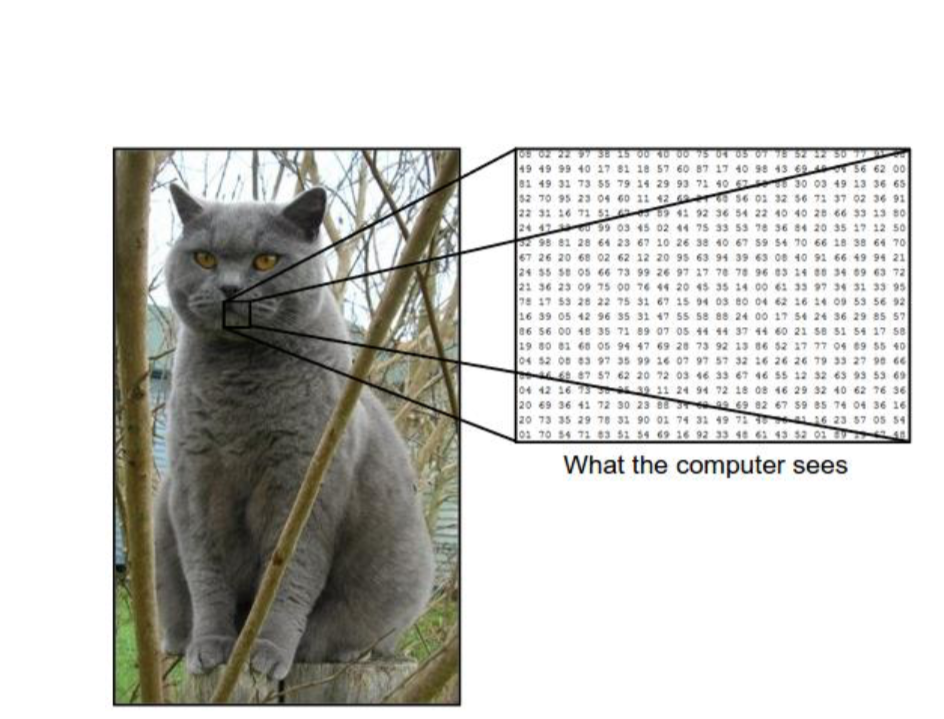
\includegraphics[width=0.7\linewidth]{figures/howcomputersees.png} 
  \caption{Representation of a cat image as a two-dimensional array of numbers.}
  \label{fig:image2d}
\end{figure}



In the late 60s, Hubel et al. discovered that the visual cortex consists of a complex arrangement of cells in the brain of cats and monkeys.  Also, these cells individually respond to specific regions.  In other words, They are more sensitive to smaller regions of the visual field - it is also called the receptive field.\\

Additionally,  in this paper two basic cell types, which act differently depending on the trigger, are described:  1) \textbf{Simple cells} activate when edge-like patterns or basic shapes like a line in their receptive field. 2) \textbf{Complex cells} are invariant to the position of a figure, so they activate whenever a known pattern is detected regardless of its position in the visual field.\\

The visual cortex of mammals being the most impressive image processing system has always been an inspiration in the computer vision community.  A few examples of many models inspired by this concept are (1) \textbf{Neocogrition} \cite{fukushima_neocognitron_2007}, in which a multi-layered artificial neural network proposed based on the concept of the Simple and Complex cells and later served as the inspiration  for CNN, and (2) \textbf{LeNet-5} \cite{lecun_gradient-based_1998} which is considered as the first Convolutional  Neural Network, and it was able to classify digits from handwritten  numbers.  In recent years, Convolutional  Neural Networks (CNN) has found its position as the most successful method to learn and  recognize patterns from images.  In the rest of this section, we introduce the basic architecture of CNNs and one of its variant, called ResNet \cite{he_deep_2015}, because we mainly focused on these two methods in this thesis.\\

The name ”convolution”  stem from convolution operation ($\circledast$) in mathematics. This is because in CNN we have filters similar to Simple cells convolved over the output array of the previous layer.   This operation allows us to find any patterns regardless of the position of it in the image, which means the convolution operation mimics the ability of Complex cells.\\

It is important to note that  there are three primary motivations for CNNs: \textbf{Sparse interaction}, \textbf{Parameter sharing}, and \textbf{Equivalence}.\\\\\\

\textbf{(a) Sparse interaction :}\\
\begin{figure}[b!]
	\centering
  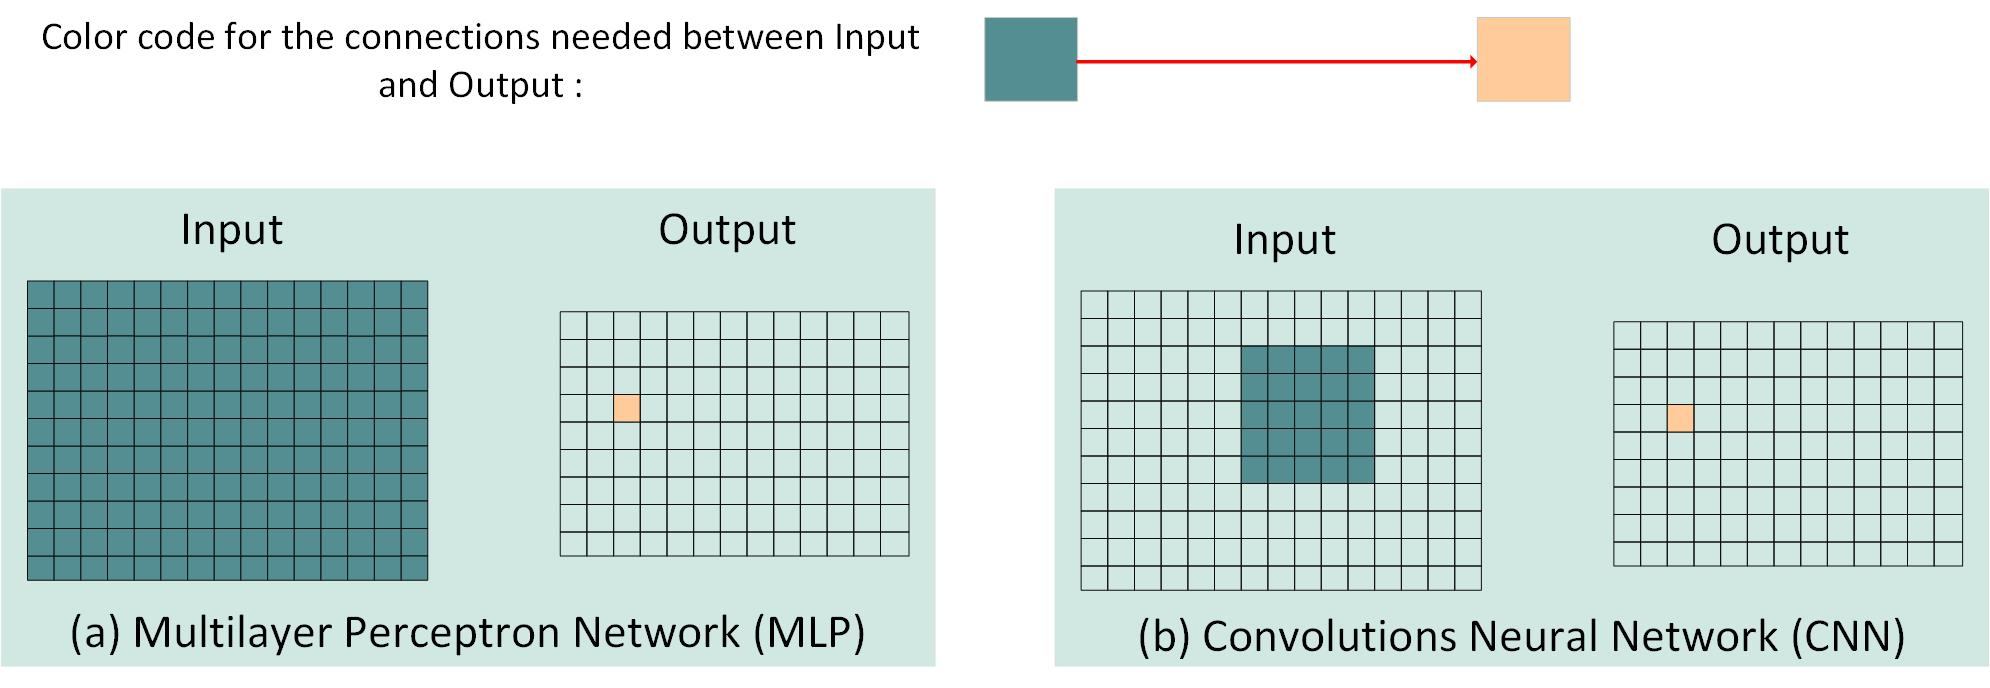
\includegraphics[width=\linewidth]{figures/mlpvscnn} 
  \caption{Comparison of MLP and CNNs in terms of number of connections needed between two layers.}
  \label{fig:mlpvscnn}
\end{figure}

Any process on images requires a lot of computational power because images naturally have bigger size compared to time-series and many other data types.  The way CNN handle this is called sparse interaction.  It is also called sparse weights since it aims to make kernels (also called as filters) smaller input.  By this, the model can have fewer parameters compared to fully-connected networks, and consequently, it reduces memory consumption and CPU operations,  and training will take much less time than training and MLP model.\\

For example, we want to compare the number of parameters to learn for MLP and CNN in case we have an input image of total m pixels (neurons)  and output of n pixels (neurons) in the following layer.  In MLP,  we need to have all m neurons to be connected to each output neuron, so as a result, we will have $m \times n$ parameters (weights).  However, for CNN, we need pixels in the ”receptive field” of size k to be connected to output pixels. In this case, we will have $k \times n$ connections, see Figure \ref{fig:mlpvscnn}. Usually $k \\ll m$, and consequently we will have much fewer operations and parameters to learn by using the concept of receptive field in the Visual cortex. \\

\textbf{(b) Parameter Sharing :}\\

As it is shown in Figure \ref{fig:prsharing}, in CNN the model only learns a set of parameters instead of learning parameters (weights)  for each of the connection like in MLP. It is clear that the number of weights, shown by annotation of W, is decreased by a factor of 4 even for an input layer of 4 neurons to a layer of 5 neurons.  Also, it is worth to note that, number of neurons is in 3 digits for image processing tasks, so parameter sharing makes a significant decrease in memory consumption. \\
\begin{figure}[h!]
	\centering
  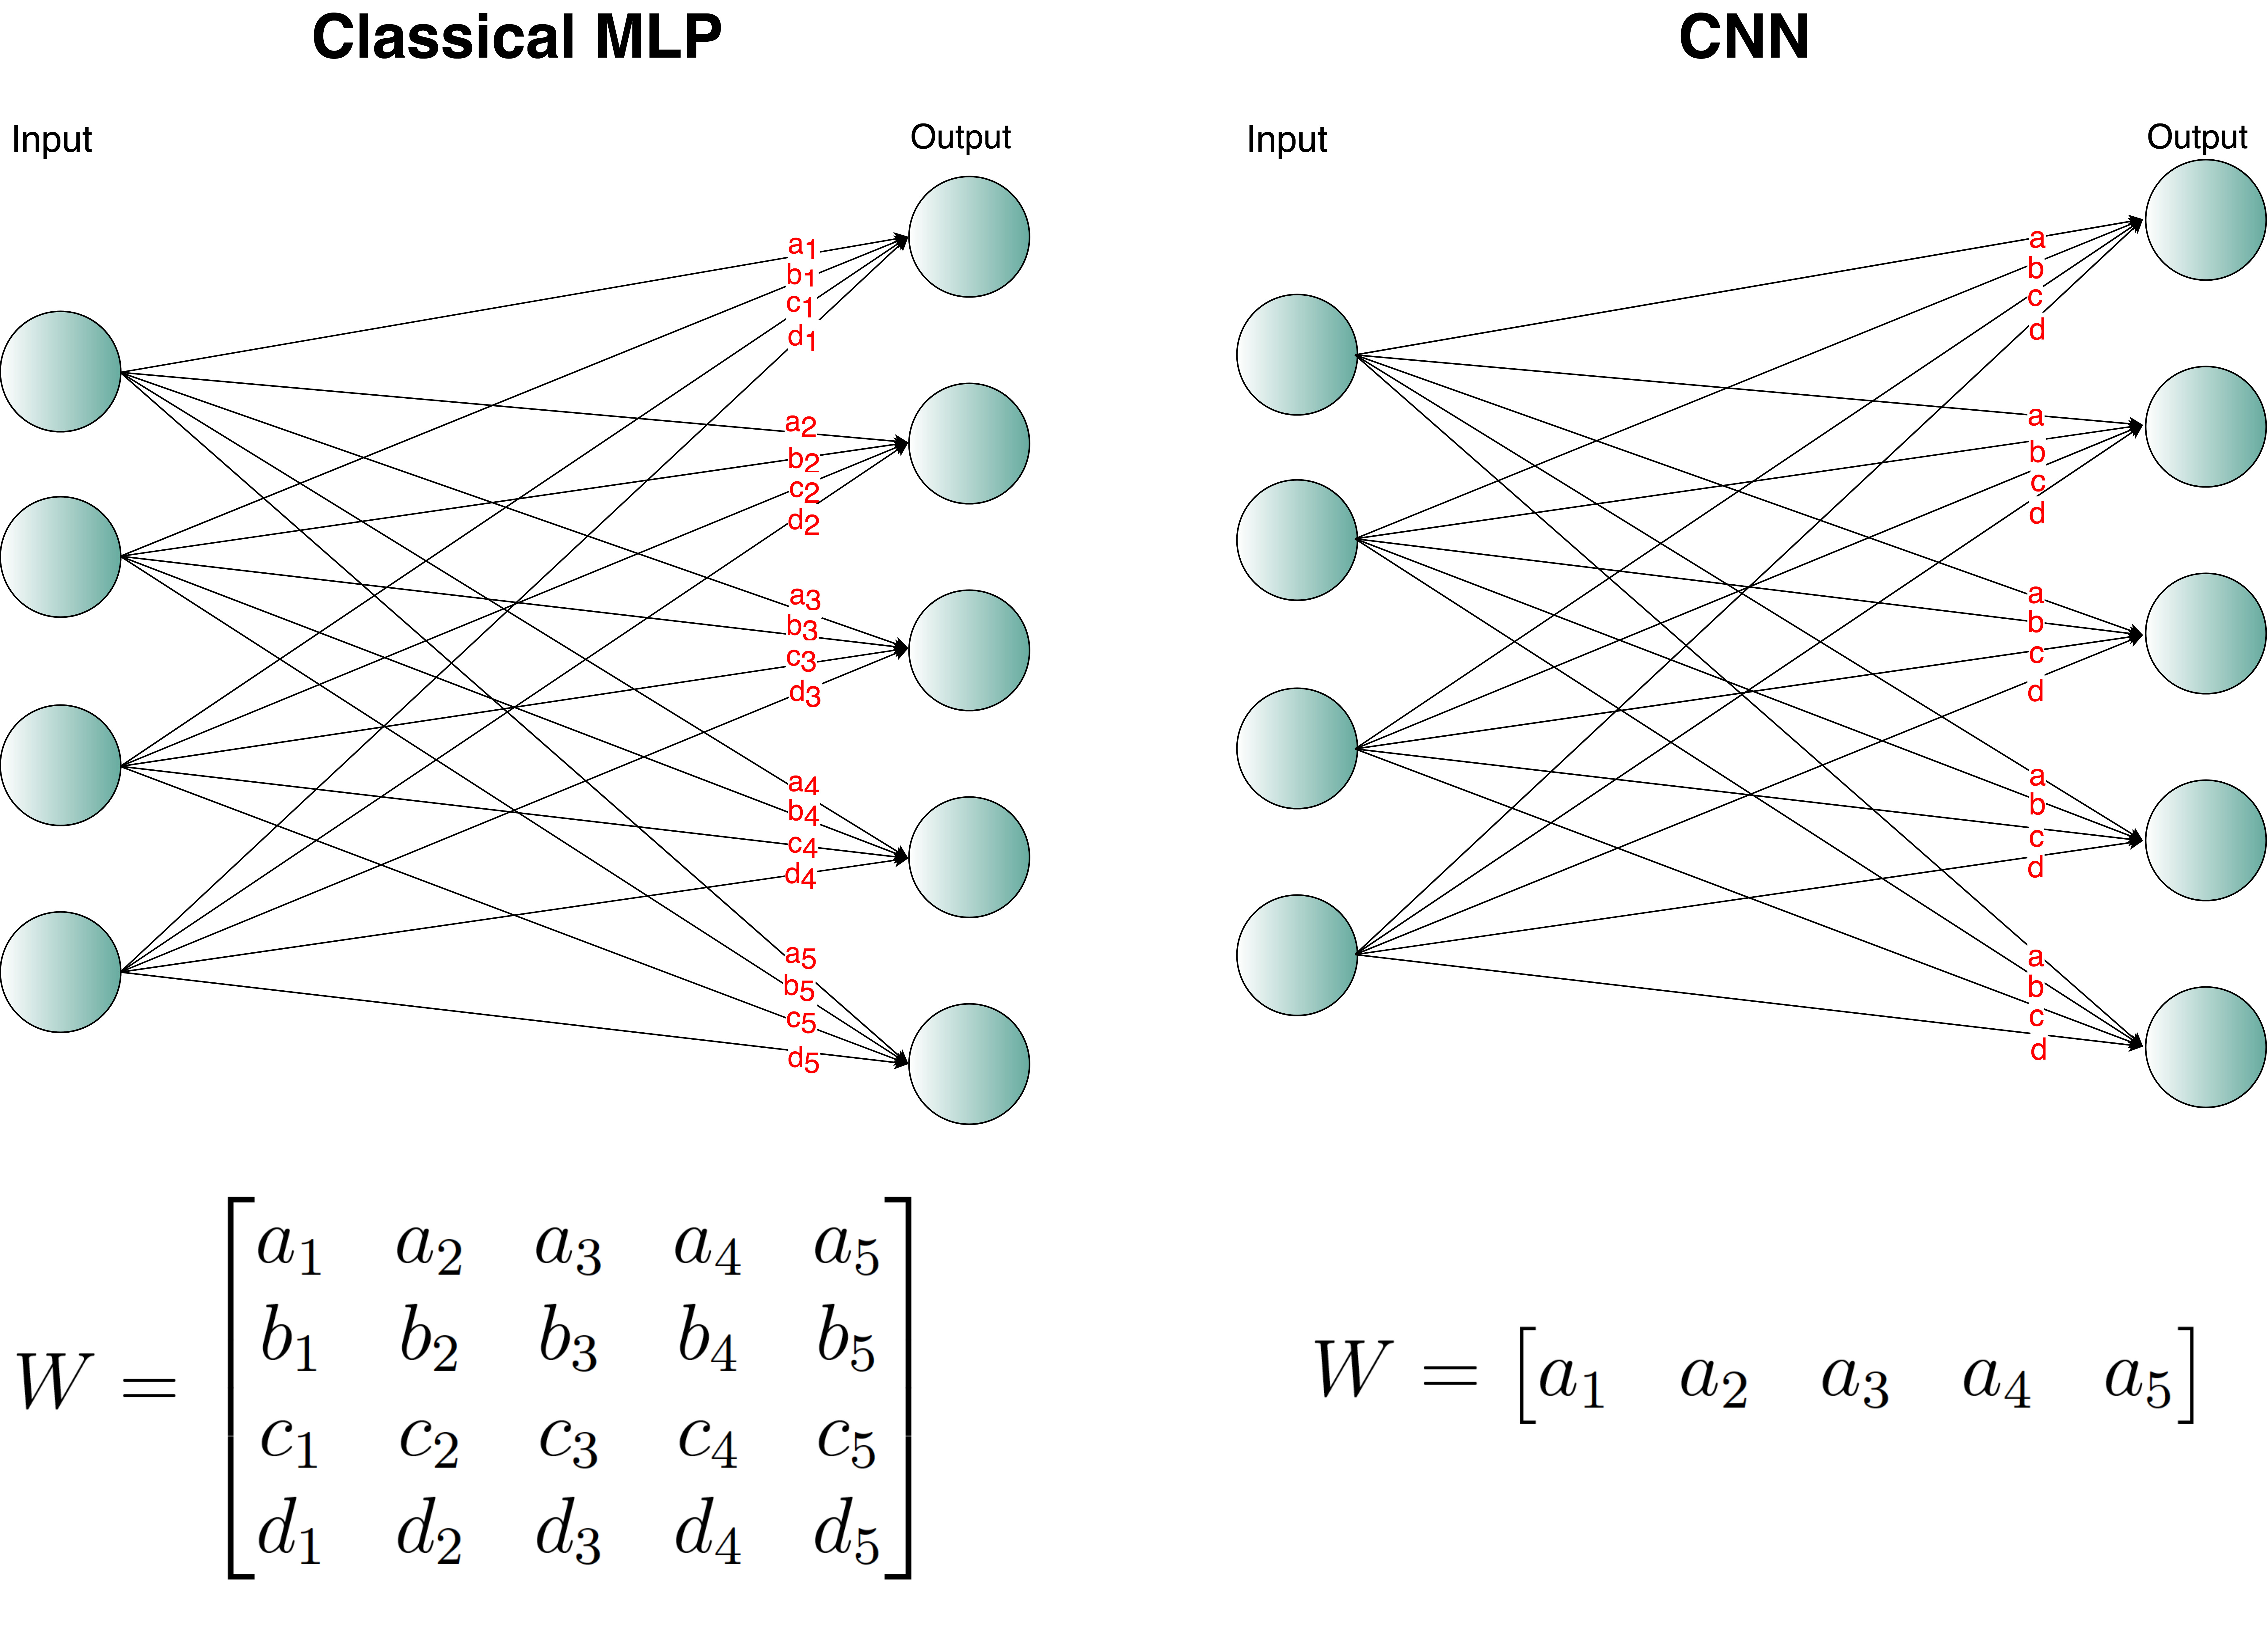
\includegraphics[width=0.8\linewidth, height=0.5\linewidth ]{figures/parameter_sharing} 
  \caption{Parameters needed in classical fully-connected network (on the left) and convolutional neural network (on the right).}
  \label{fig:prsharing}
\end{figure}
\clearpage
\textbf{(c) Equivalence :}\\

if  $f(g(x)) = g(f(x))$, then $f(x)$ is equivalent to g.  For example, CNN is equivalent to translation in images, meaning that any change in the position of an object in the image is observed in the output in the same manner.  This property is different from invariance.
\begin{itemize}
\item \textbf{Invariance} means the  internal  representation of an object  does not  change when the properties  of that  object change, $f(g(x)) = f(x)$,
\item \textbf{Equivalence} means  the  internal  representation captures  the  properties  of the object, $f(g(x)) = g(f(x))$. 
\end{itemize}

In CV tasks, there are three main operations where algorithms aim to be invariant to translation, scaling, and rotation.  CNN only brings equivalence to the solution. However, with the help of max pooling operation after convolution operation we can solve the problem of invariance.  For the sake of simplicity, we investigate 2D convolutional neural networks (CNNs) architecture in the rest of this section. \\
\begin{figure}[t!]
	\centering
  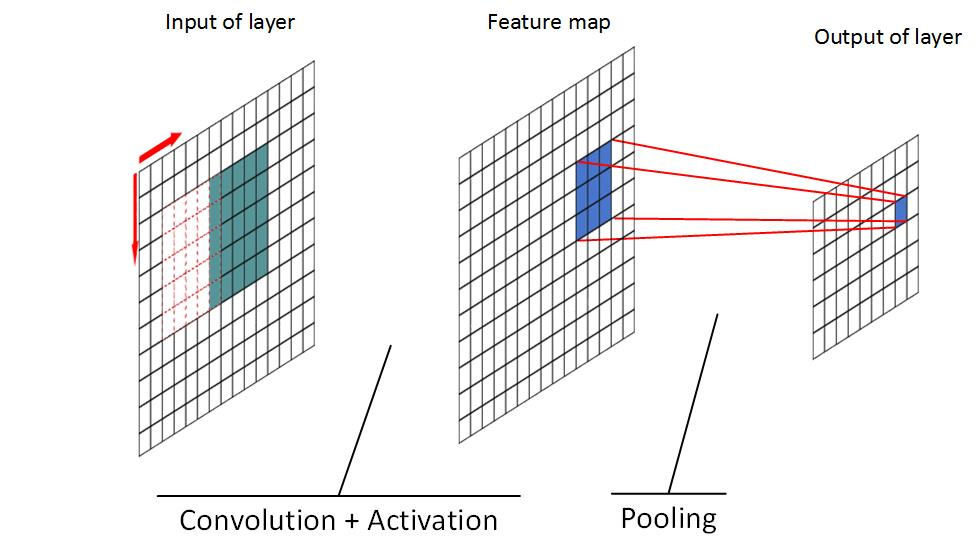
\includegraphics[width=0.8\linewidth]{figures/cnn_stages}  
  \caption{A basic convolutional layer, which consists of a convolution operation followed by an activation, and at the end pooling (a popular example is  max-pooling) operation is applied. It can be observed that the size of input image is shallowed.}
  \label{fig:cnnstages}
\end{figure}

Convolutional neural networks is essentially a variant of fully connected Multilayer perceptron network (MLP). In the sense of the layer structure and operations between input and neuron weights except for convolution, and pooling operations.  In both of networks, data flow forward, unlike recurrent neural networks (RNN), through weights, and the core functionality is done by a simple dot product between weights and input. Besides, in both types of these networks the resulting outcome of dot product pass through an activation function as shown in Equation  \ref{eq:dot}, such as ReLu, sigmoid, or tanh.  In Figure \ref{fig:mlpvscnn}, one significant difference between CNNs and MLP is shown, which is that in CNN the connections between input and output is local but in MLP it is fully connected regardless of the region of the input data \cite{lecun_gradient-based_1998}.\\

\begin{equation}
\label{eq:dot}
\begin{aligned}
  a_{xy} =& \sum\limits_{i}\sum\limits_{j}(w_{ij}\cdot v_{x+i,y+j} + b),\\
  z_{xy} =& f(a_{xy}),
\end{aligned}
\end{equation}

in which $v_{x+i,y+j}$ is input at the position $(x+i,y+j)$, b is the bias term, $w_{ij}$ weight of the kernel at position $(i,j)$, $a_{x,y}$ is the output of the summation at $(x,y)$, $f(..)$ is an \textit{activation function}, and lastly $z_{xy}$ is the output at position $(x,y)$, $z$ as a whole is also called \textit{feature map}. \\

One layer of CNN mainly consists of 3 stages:   convolution,  activation, and pooling stages see Figure \ref{fig:cnnstages}. Convolution layer, as the name implies, convolve a kernel (filter) of specified size than input over the input image. Later it is fed into an activation function, Usually Rectified Linear Unit (ReLu) activation function shown in Figure \ref{fig:activations}\footnote{\url{https://cdn-images-1.medium.com/max/1200/1*ZafDv3VUm60Eh10OeJu1vw.png}}. After that, a pooling operation is performed over a specified size.  This operation is quite similar to convolution operations except we do not have any parameters to learn in this stage unlike in convolution stage.\\

\begin{figure}[h!]
	\centering
  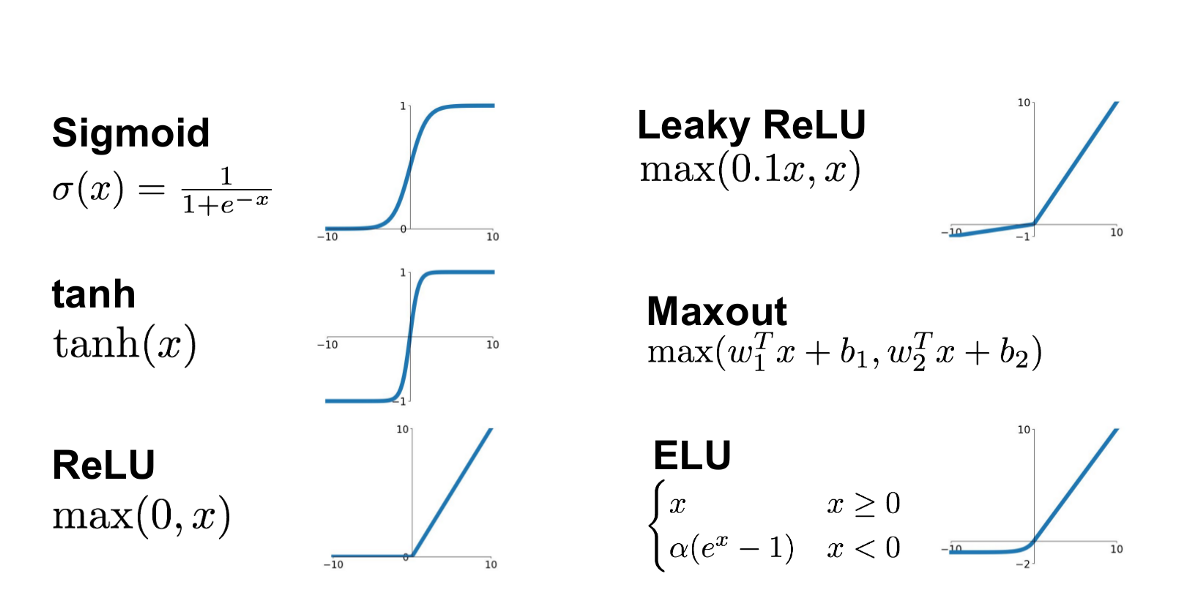
\includegraphics[width=0.8\linewidth]{figures/activations.png} 
  \caption{Some examples of activations functions.}
  \label{fig:activations}
\end{figure}

As I mentioned before, there are three transformations in images need to be tackled in CV tasks.  These are scaling, rotation and translation.  The convolution and pooling operations handle translation since it mimics the "receptive field" concept\footnote{\url{http://cs231n.github.io/}} by creating local connections between input and feature map.  Scaling problem,  on the other hand, is been solved pooling operation,  which maps a 2-dimensional subregion of feature map to one value.  Two most popular pooling strategies have proved to work well are \textit{Max Polling} and \textit{Average Pooling}.  Lastly, the rotation could be only achieved by either increasing samples from different angles in the training data or applying some augmentation methods.  It is important to note that  , augmentation methods  can work for scaling and translation as well and improve the performance a lot.\\

\begin{figure}[t!]
	\centering
  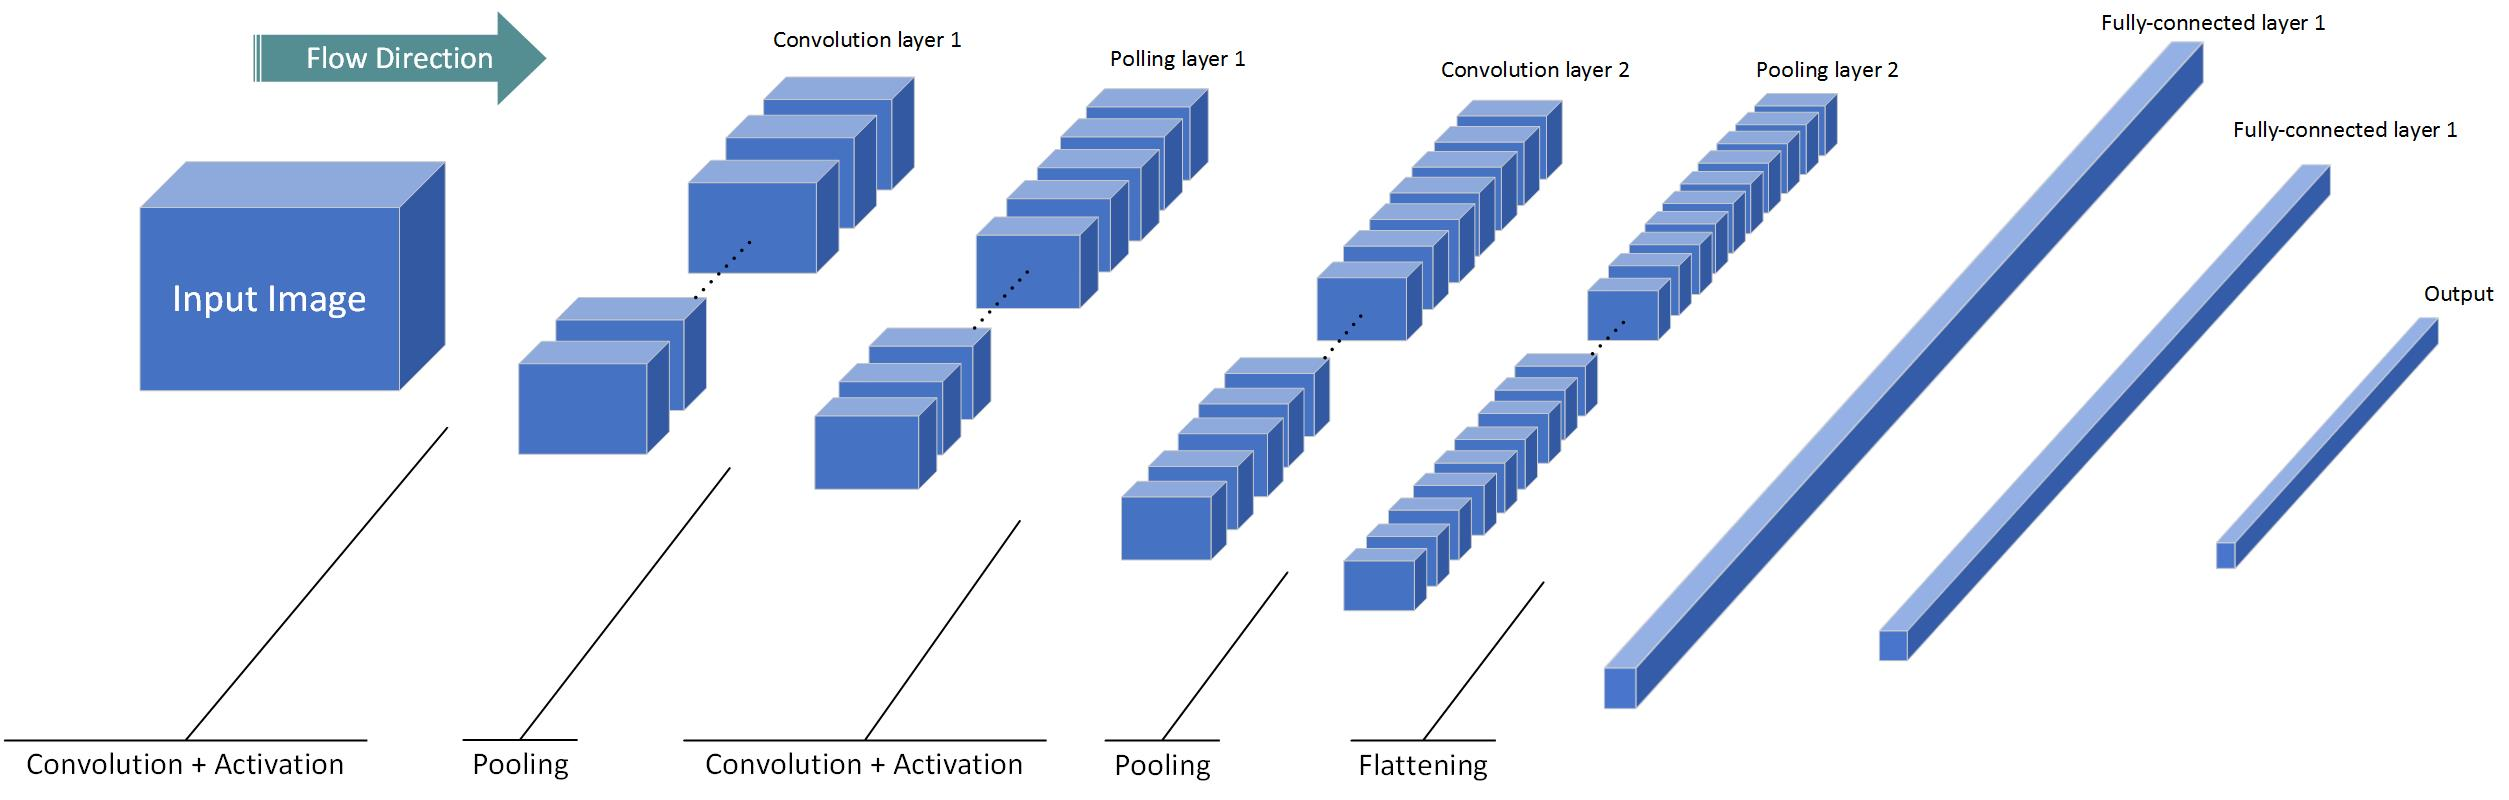
\includegraphics[width=\linewidth]{figures/cnn_whole} 
  \caption{An example of convolutional neural network model on images. It consists of two concolutional layer, and 3 fully connected layer on top of it. The last layer of the model should have a size equal to the number of classes.}
  \label{fig:cnn_whole}
\end{figure}

The general structure of a Convolutional neural network (CNN) with two convolution layers, each followed by a pooling layer, and two fully-connected layers are shown in Figure \ref{fig:cnn_whole}.  As I mentioned before, CNN is a powerful feature  extractor, and the responsible layers for feature extraction are convolution layers. In the end, we assume that the right features are created and on top of it any machine learning method can be applied. Although this is the case, most of the times this machine learning method is a fully-connected multilayer perceptron network (MLP)  as it is shown in Figure \ref{fig:cnn_whole} because we can train our network  on the fly with this structure.  Imagine if we want to use a Support  Vector  Machine (SVM), then we cannot train the whole network as a whole, instead we need first to train a CNN + MLP network and then use only convolution layers’ output to train an SVM.\\


Besides this structure, there are many other CNN-inspired methods developed.  One of the most powerful one recently developed by K. He and X. Zhang is ResNet \cite{he_deep_2015}. ResNet stands for Residual Network, and the idea of this paper is bypassing the input to the output of two consequtive convolution layer.  By doing so, it allows back-propagation from output to the input more efficient and solves the vanishing gradient problem, which is a phenomena happens when gradient converges to zero as the number of layers increases in the network.\\

In Figure \ref{fig:blocks}, basic residual blocks of ResNet (at the left side) and ResNext (at the right side) are shown. A ResNet block has two convolutional layers followed by a batch normalization and a ReLU activation.   Like all residuals block, there is a connection between input and output between second batch normalization and ReLU operation.    This structure is first introduced in \cite{he_deep_2015}, and it allows for training networks with more than 100 layers.    This revolutionized Computer   Vision/  Deep Learning community as training deep networks is one of the main challenges. In \cite{he_identity_2016}, researchers achieved to train even 1001-layered ResNet.   Because of its appealing results in many tasks, ResNet quickly became popular in the research community.  There are many variants of ResNet developed in  3 years by changing the structure of the residual block.  In ResNext, the residual block has many parallel convolutions and one bypass connection from the input to the output.  One of the most successful ones is called ResNext whose basic block is shown at the right side of Figure \ref{fig:blocks}, and in this thesis, we will use ResNext-101 \cite{xie_aggregated_2016} and C3D \cite{tran_learning_2014}, which is also a well-known 3D CNN architecture,  as our classifiers. ResNet-10, on the other hand,  will be used for the detection of gestures as it has a relatively much smaller structure as detection task does not require a complex and heavy model. \\


